\documentclass[a4paper]{article}
\usepackage[T1]{fontenc}			% pacchetto per \chapter
\usepackage[italian]{babel}
\usepackage[italian]{isodate}  		% formato delle date in italiano
\usepackage{graphicx}				% gestione delle immagini
\usepackage{amsfonts}
\usepackage{booktabs}				% tabelle di qualità superiore
\usepackage{amsmath}				% pacchetto matematica
\usepackage{mathtools}				% per sottolineare sotto le equazioni
\usepackage{stmaryrd} 				% per '\llbracket' e '\rrbracket'
\usepackage{amsthm}					% teoremi migliorati
\usepackage{enumitem}				% gestione delle liste
\usepackage{pifont}					% pacchetto con elenchi carini
\usepackage{enumitem}				% pacchetto per elenchi con lettere dell'alfabeto
\usepackage{cancel}					% per cancellare delle espressioni matematiche
\usepackage{caption}				% caption personalizzati
\usepackage[]{mdframed}				% box per il testo
\usepackage{multirow}				% più linee in una tabella
\usepackage{gensymb}				% simbolo di degree


% draw a frame around given text
\newcommand{\framedtext}[1]{%
	\par%
	\noindent\fbox{%
		\parbox{\dimexpr\linewidth-2\fboxsep-2\fboxrule}{#1}%
	}%
}



\usepackage[x11names]{xcolor}		% pacchetto colori RGB
% Link ipertestuali per l'indice
\usepackage{xcolor}
\usepackage[linkcolor=black, citecolor=blue, urlcolor=cyan]{hyperref}
\hypersetup{
	colorlinks=true
}

\usepackage{tikz}
\newcommand{\MyTikzmark}[2]{%
	\tikz[overlay,remember picture,baseline] \node [anchor=base] (#1) {#2};%
}
\newcommand{\DrawVLine}[3][]{%
	\begin{tikzpicture}[overlay,remember picture]
		\draw[shorten <=0.3ex, #1] (#2.north) -- (#3.south);
	\end{tikzpicture}
}
\newcommand{\DrawHLine}[3][]{%
	\begin{tikzpicture}[overlay,remember picture]
		\draw[shorten <=0.2em, #1] (#2.west) -- (#3.east);
	\end{tikzpicture}
}


%\usepackage{showframe}				% visualizzazione bordi
%\usepackage{showkeys}				% visualizzazione etichetta

\newtheorem{theorem}{\textcolor{Red3}{\underline{Teorema}}}
\newtheorem{lemma}{Lemma}
\renewcommand{\qedsymbol}{QED}
\newcommand{\exec}[1]{\llbracket #1\:\rrbracket}
\newcommand{\dquotes}[1]{``#1''}
\newcommand{\longline}{\noindent\rule{\textwidth}{0.4pt}}
\newcommand{\circledtext}[1]{\raisebox{.5pt}{\textcircled{\raisebox{-.9pt}{#1}}}}

\newenvironment{rowequmat}[1]{\left(\array{@{}#1@{}}}{\endarray\right)}
\newenvironment{rowequmatbra}[1]{\left[\array{@{}#1@{}}}{\endarray\right]}

\begin{document}
	\author{VR443470}
	\title{Guida agli Esami di Linguaggi}
	\date{\printdayoff\today}
	\maketitle
	
	\newpage
	
	% indice
	\tableofcontents
	
	\newpage
	
	\section{Esercizio 1 - Domanda di teoria su Interprete e Compilatore}
	
	\subsection{Interprete}
	
	In molti esami si presenta la richiesta della definizione di interprete. Nonostante possa essere banale, viene richiesto un \dquotes{alto} livello di approfondimento dato che vale ben 4 punti all'interno dell'esame. In ogni caso, è possibile affermare che questa domanda sia una delle più gettonate.\newline
	
	\noindent
	\textcolor{Red3}{\textbf{\emph{Definire intuitivamente e formalmente (mediante definizione semantica) cosa è un interprete. Descrivere la struttura di un interprete e spiegarne il funzionamento.}}}\newline
	
	\noindent
	\textcolor{Green4}{\textbf{\emph{\underline{Risposta}}}}\newline
	
	\noindent
	La definizione intuitiva di un interprete è la seguente.
	
	Un \textbf{interprete} è un programma $\mathrm{int}^{L_{0}, L}$ che esegue, sulla macchina astratta per $L_{0}$, programmi $P^{L}$, i quali sono scritti nel linguaggio di programmazione $L$, su un input fissato appartenente all'insieme dei dati $D$ (input e output).\newline
	Utilizzando parole povere, un interprete non è altro che una \dquotes{macchina universale} che preso un programma e un suo input, esegue (il programma) sul quel determinato input usando \underline{soltanto} le funzionalità messe a disposizione dal livello (macchina astratta) sottostante.
	\begin{mdframed}
		\emph{Un attimo, ma che cosa si intende per livello? E macchina astratta?} Cerchiamo di fare chiarezza.\newline
		
		\noindent
		Dato un linguaggio di programmazione $L$, la \underline{macchina astratta} $M_{L}$ per $L$ è un insieme di strutture dati ed algoritmi che consentono di memorizzare ed eseguire programmi scritti in $L$. La sua realizzazione può essere fatta in Hardware, Firmware o Software.\newline
		
		\noindent
		\emph{Si ma quindi cosa si intende per livello?}\newline
		
		\noindent
		Con la scelta della categoria \dquotes{realizzazione software}, vengono utilizzati, per la realizzazione di strutture dati e algoritmi, linguaggi di programmazione ad alto livello poiché essi implementano una struttura suddivisa a \underline{livelli} di astrazione.\newline
		Per concludere, la macchina astratta può essere dunque vista come una stratificazione di livelli dove ciascuno di essi coopera in modo sequenziale, ma allo stesso tempo è indipendente.\newline
		
		\noindent
		Per non lasciare niente al caso, con \dquotes{\underline{linguaggio di programmazione ad alto} \underline{livello}} ci si riferisce a tutti quei linguaggi di programmazione che offrono un livello di astrazione molto alto dei dettagli del funzionamento del calcolatore.
	\end{mdframed}\newpage
	
	\noindent
	Prima della definizione formale di interprete, si illustrano due notazioni necessarie:
	\begin{itemize}
		\item Con il termine $Prog^{L}$ ci si riferisce all'insieme dei programmi scritti nel linguaggio di programmazione $L$;
		
		\item Con la dicitura:
		\begin{equation*}
			\exec{P^{L}} \: : \: D \rightarrow D
		\end{equation*}
		Si indica che l'esecuzione del programma scritto nel linguaggio di programmazione $L$ ($\exec{P^{L}}$) con input $in$ è uguale all'output $out$. Ovverosia:
		\begin{equation*}
			\exec{P^{L}}\left(in\right) = out	
		\end{equation*}
	\end{itemize}
	Un \textbf{interprete formalmente} è descrivibile nel seguente modo. Si consideri un interprete da $L$ a $L_{0}$: dato $P^{L} \in Prog^{L}$ e $in \in D$, un interprete $int^{L, L_{0}}$ per $L$ su $L_{0}$ è un programma tale che:
	\begin{equation*}
		\exec{int^{L, L_{0}}} \: : \: \left(Prog^{L}\right) \rightarrow D
	\end{equation*}
	Ne consegue che:
	\begin{equation*}
		\exec{int^{L, L_{0}}} \: : \: \left(P^{L}, in\right) = \exec{P^{L}}\left(in\right)
	\end{equation*}
	\begin{figure}[!htp]
		\centering
		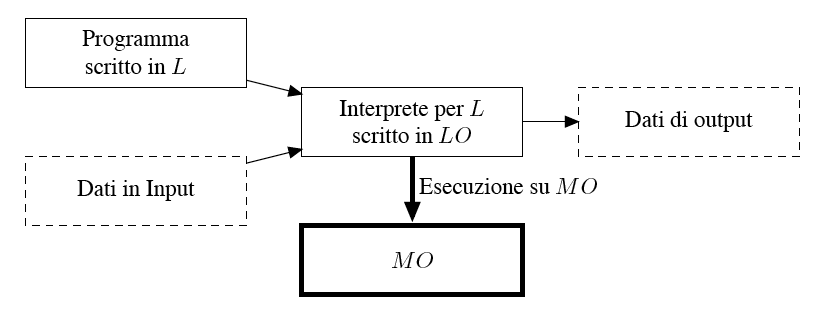
\includegraphics[width=\textwidth]{img/ex1-1.png}
		\caption*{Riassunto visivo di quanto appena descritto.}
	\end{figure}\newpage
	
	\noindent
	Qua di seguito si presenta il ciclo di esecuzione di un interprete:
	\begin{figure}[!htp]
		\centering
		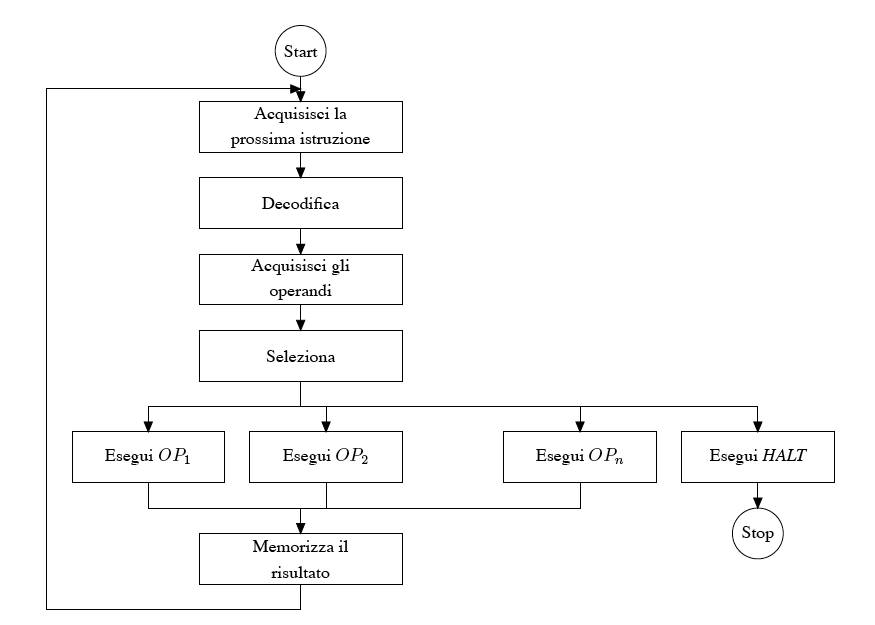
\includegraphics[width=\textwidth]{img/ex1-2.png}
	\end{figure}
	\begin{enumerate}
		\item Il ciclo di esecuzione di un interprete si apre con l'acquisizione di un'istruzione da eseguire;
		
		\item L'operazione del passo precedente viene decodificata;
		
		\item Nel caso in cui l'operazione abbia bisogno di operandi, anch'essi vengono acquisiti dalla memoria;
		
		\item Data l'operazione acquisita al passo 1, viene selezionata una determinata operazione: nel caso di $OP_{...}$ si esegue un'operazione, nel caso di $HALT$ l'esecuzione di un interprete si ferma;
		
		\item Dopo l'operazione eseguita, se vi è un risultato, esso viene salvato. In ogni caso, il ciclo inizia nuovamente la sua esecuzione.
	\end{enumerate}
	
	\newpage
	\subsection{Compilatore}
	
	Non è frequente la richiesta della definizione di compilatore, ma rimane una domanda di teoria che può essere richiesta.\newline
	
	\noindent
	\textcolor{Red3}{\textbf{\emph{Definire intuitivamente e formalmente (mediante definizione semantica) cosa è un compilatore. Descrivere e spiegare poi la struttura di un compilatore (preferibilmente come flow-chart).}}}\newline
	
	\noindent
	\textcolor{Green4}{\textbf{\emph{\underline{Risposta}}}}\newline
	
	\noindent
	La definizione intuitiva di un compilatore è la seguente.
	
	Un \textbf{compilatore} è un programma $comp^{L_{0},L}$ che traduce, preservando semantica e funzionalità, programmi scritti nel linguaggio di programmazione $L$ in programmi scritti in $L_{0}$, e quindi eseguibili direttamente sulla macchina astratta per $L_{0}$.\newline
	
	\noindent
	Dato un linguaggio di programmazione $L$, una macchina astratta $M_{L}$ per $L$ è un insieme di strutture dati e algoritmi che consentono la memorizzazione e l'esecuzione dei programmi scritti nel linguaggio di programmazione $L$ ($P^{L}$).\newline
	
	\noindent
	Prima di dare la definizione formale di interprete, si forniscono alcune notazioni:
	\begin{itemize}
		\item $Prog^{L}$ è un insieme di programmi scritti nel linguaggio di programmazione $L$;
		\item $D$ è l'insieme dei dati (input e output);
		\item $P^{L}$ è il programma scritto nel linguaggio di programmazione $L$;
		\item $\exec{P^{L}} \: : \: D \rightarrow D$ rappresenta la semantica di $P^{L}$, ovvero l'esecuzione del programma nel linguaggio di programmazione $L$ con input $in$ è uguale all'output $out$:
		\begin{equation*}
			\exec{P^{L}}(in) = (out)
		\end{equation*}
	\end{itemize}
	La definizione formale di un compilatore è la seguente.
	
	Dato $P^{L} \in Prog^{L}$, un \textbf{compilatore formalmente} $comp^{L,L_{0}}$ da $L$ a $L_{0}$ è un programma che:
	\begin{equation*}
		\exec{comp^{L,L_{0}}}: Prog^{L} \rightarrow Prog^{L_{0}}
	\end{equation*}
	Ovvero:
	\begin{equation*}
		\exec{comp^{L,L_{0}}}\left(P^{L}\right) = \left(P^{L_{0}}\right) \hspace{1em} \text{tale che} \hspace{1em} \forall in \in D.\exec{P^{L_{0}}}\left(in\right) = \exec{P^{L}}\left(in\right)
	\end{equation*}
	In linguaggio non matematico, significa che l'esecuzione del compilatore da $L$ a $L_{0}$ insieme (input) ad un determinato programma scritto in un linguaggio di programmazione $L$ è uguale (output) al programma scritto nel linguaggio di programmazione $P^{L_{0}}$; tale che per ogni input $in$ appartenente all'insieme dei dati $D$, l'esecuzione di un programma scritto nel linguaggio di programmazione $L_{0}$ con input $in$ è uguale all'esecuzione del programma scritto nel linguaggio di programmazione $L$ con input $in$.\newpage
	
	\begin{figure}[!htp]
		\centering
		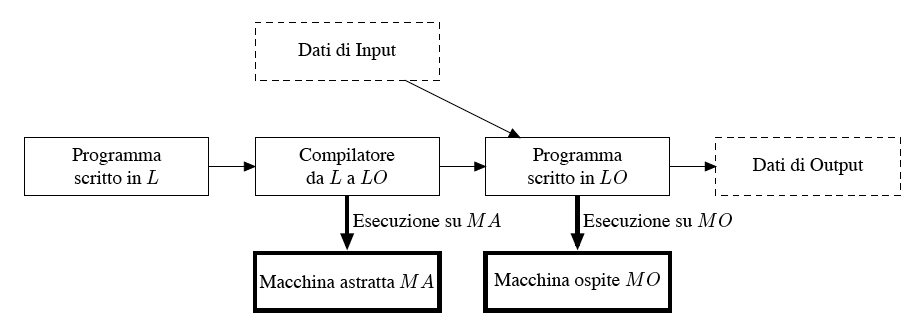
\includegraphics[width=\textwidth]{img/ex1-3.png}
		\caption*{Flow-chart di quanto detto precedentemente.}
	\end{figure}
	
	\noindent
	Si presenta qua di seguito la \textbf{struttura di un compilatore}:
	\begin{figure}[!htp]
		\centering
		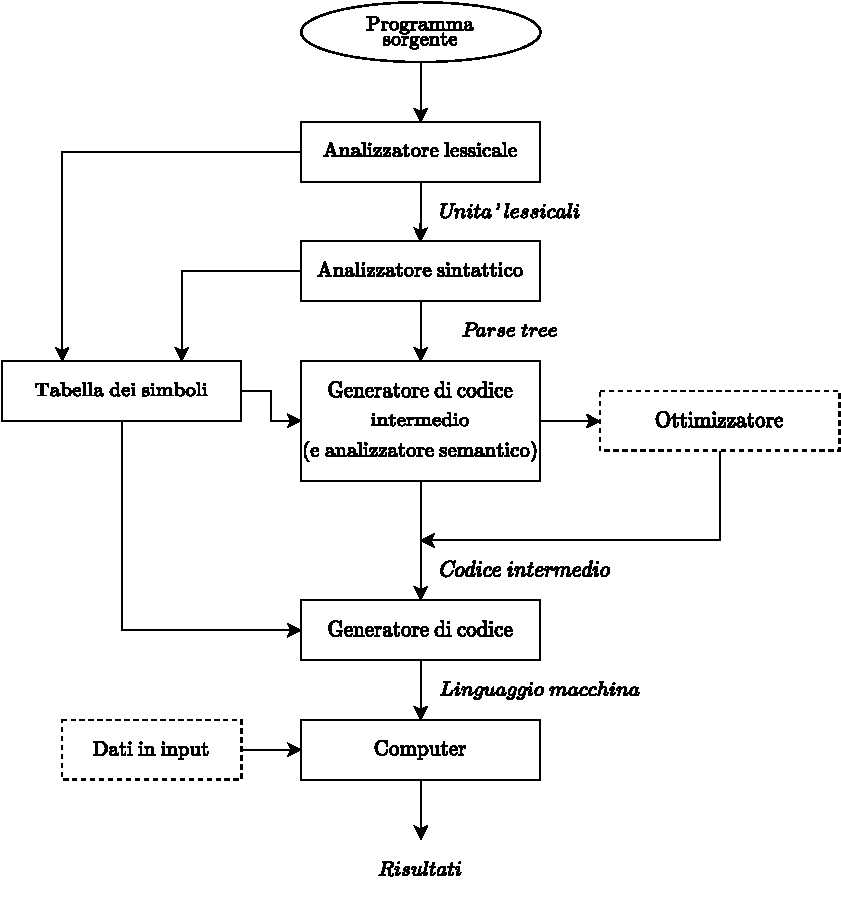
\includegraphics[width=\textwidth]{img/ex1-4.pdf}
	\end{figure}\newpage
	
	\begin{enumerate}
		\item Il programma sorgente, da compilare, passa in prima battuta da un analizzatore lessicale. Vengono \textbf{convertiti i caratteri del programma sorgente in unità lessicali}. Quest'ultime possono essere \emph{identificatori}, \emph{numeri}, \emph{parole riservate} e formano i linguaggi regolari.
		
		\item Le unità lessicali finiscono in un analizzatore sintattico, il quale crea una albero che rappresenta la sintassi del programma:
		\begin{itemize}
			\item Le foglie (\emph{token}) vengono lette da sinistra verso destra e costituiscono le frasi ben formate del linguaggio;
			
			\item Dal precedente punto, ne consegue che l'impossibilità della costruzione di un albero è dovuta all'illegalità di quale frase (mal formata, errore di compilazione!);
		\end{itemize}
		Quindi, l'\textbf{analizzatore sintattico trasforma unità lessicali in \emph{parse tree} (albero di parse) che rappresentano la struttura sintattica del programma}.
		
		\item Riceve informazioni dall'analizzatore lessicale/sintattico e \textbf{memorizza informazioni sui nomi presenti nel programma} (identificatori, chiamate di procedura, ecc.);
		
		\item A questo punto, viene \textbf{generato un codice intermedio} che è \emph{indipendente dall'architettura}, e vengono \textbf{rilevati eventuali errori semantici} grazie all'\emph{analizzatore semantico};
		
		\item (Opzionale) Il codice può essere ottimizzato in questa fase;
		
		\item Si conclude la struttura del compilatore con la generazione del codice macchina che, a differenza del codice intermedio, è dipendente dall'architettura.
	\end{enumerate}
	La parte finale dello schema mostra l'esecuzione del programma compilato su un computer con eventuali dati in input.\newpage
	
	\section{Esercizio 2 - Induzione}
	
	\subsection{Dimostrare $\forall n \in \mathbb{N}.n + n^{2}$ è un numero pari}
	
	\textcolor{Red3}{\textbf{\emph{Dimostrare per induzione che $\forall n \in \mathbb{N}.n + n^{2}$ è un numero pari.}}}\newline
	
	\noindent
	\textcolor{Green4}{\textbf{\emph{\underline{Risposta}}}}\newline
	
	\noindent	
	L'\textbf{induzione} è una tecnica di dimostrazione che consente di dimostrare la validità di una tesi dalla verifica di due condizioni: la validità della \dquotes{base induttiva} e la validità del \dquotes{passo induttivo}.
	\begin{proof}[\textbf{Caso base}]
		Si sceglie come caso base il valore $n = 1$. Si sostituisce:
		\begin{equation*}
			\begin{array}{rcl}
				n + n^{2} &\rightarrow& \text{ è pari? } \textcolor{Green4}{\checkmark} \\ [.3em]
				&\downarrow& \text{sostituzione di }n=1 \\ [.3em]
				1 + 1^{2} = 2 &\rightarrow& \text{ è pari? } \textcolor{Green4}{\checkmark}
			\end{array}
		\end{equation*}
		Utilizzando un linguaggio più formale, utile per la dimostrazione, è anche possibile affermare che il modulo di $n+n^{2}$ diviso $2$ è uguale a zero. Ovvero, che dividendo un numero pari per $2$ (per definizione), si ottiene il valore zero:
		\begin{equation*}
			\begin{array}{rcl}
				n+n^{2} &=& 0 \: \left(\mathrm{mod} \: 2\right) \\ [.3em]
				%
				&\downarrow& \text{sostituzione di }n=1 \\ [.3em]
				%
				1+1^{2} &=& 0 \: \left(\mathrm{mod} \: 2\right)
			\end{array}
		\end{equation*}
	\end{proof}
	
	\noindent
	\textbf{\emph{Ipotesi induttiva:}} si assume che sia vera:
	\begin{equation*}
		n+n^{2} = 0 \: \left(\mathrm{mod} \: 2\right) \hspace{1em} \forall n \in \mathbb{N}
	\end{equation*}
	
	\begin{proof}[\textbf{Passo induttivo}]
		Si dimostra che l'ipotesi induttiva implica la validità della proprietà per $n+1$:
		\begin{equation*}
			\begin{array}{rcl}
				n+n^{2} &=& 0 \: \left(\mathrm{mod} \: 2\right) \\ [.3em]
				%                                                       
				&\downarrow& \text{applico passo induttivo} \\ [.3em]    
				%
				n+1 + \left(n+1\right)^{2} &=& 0 \: \left(\mathrm{mod} \: 2\right) \\ [.3em]
				%
				n + 1 + n^{2} + 2n + 1 &=& 0  \: \left(\mathrm{mod} \: 2\right) \\ [.3em]
				%
				n^{2} + n + 2n + 2 &=& 0 \: \left(\mathrm{mod} \: 2\right) \\ [.3em]
				%
				&\downarrow& \text{applico l'ipotesi induttiva} \\ [.3em]
				%
				n^{2} + n + 2n + 2 &=& n^{2} + n \\ [.3em]
				%
				2n + 2 &=& 0 \: \left(\mathrm{mod} \: 2\right)
			\end{array}
		\end{equation*}
		Per definizione:
		\begin{itemize}
			\item Qualsiasi numero moltiplicato per $2$ si ottiene un numero pari;
			\item Il risultato tra la somma di due numeri pari è ancora un numero pari.
		\end{itemize}
	\end{proof}\newpage
	
	\subsection{Dimostrare $\displaystyle\sum_{i=1}^{n}\dfrac{1}{i\left(i+1\right)} = \dfrac{n}{n+1}$}
	\textcolor{Red3}{\textbf{\emph{Dimostrare per induzione che }}$\displaystyle\sum_{i=1}^{n}\dfrac{1}{i\left(i+1\right)} = \dfrac{n}{n+1}$\textbf{\emph{.}}}\newline
	
	\noindent
	\textcolor{Green4}{\textbf{\emph{\underline{Risposta}}}}\newline
	
	\noindent
	L'\textbf{induzione} è una tecnica di dimostrazione che consente di dimostrare la validità di una tesi dalla verifica di due condizioni: la validità della \dquotes{base induttiva} e la validità del \dquotes{passo induttivo}.
	\begin{proof}[\textbf{Caso base}]
		Si sceglie come caso base il valore $n = 1$. Quindi, si va a sostituire:
		\begin{equation*}
			\begin{array}{rcl}
				\displaystyle\sum_{i=1}^{n}\dfrac{1}{i\left(i+1\right)} &=& \dfrac{n}{n+1} \\ [1.5em]
				%
				&\downarrow& \text{sostituzione }n=1 \\ [.5em]
				%
				\displaystyle\sum_{i=1}^{1}\dfrac{1}{i\left(i+1\right)} &=& \dfrac{1}{1+1} \\ [1.5em]
				%
				&\downarrow& \text{calcolo della sommatoria} \\ [.5em]
				%
				\displaystyle\sum_{i=1}^{1}\dfrac{1}{1\left(1+1\right)} &=& \dfrac{1}{1+1} \\ [1.5em]
				%
				\dfrac{1}{2} &=& \dfrac{1}{2}
			\end{array}
		\end{equation*}
	\end{proof}
	
	\noindent
	\textbf{\emph{Ipotesi induttiva:}} si assume che sia vera:
	\begin{equation*}
		\displaystyle\sum_{i=1}^{n}\dfrac{1}{i\left(i+1\right)} = \dfrac{n}{n+1} \hspace{2em} \forall n
	\end{equation*}
	
	\begin{proof}[\textbf{Passo induttivo}]
		Si dimostra che l'ipotesi induttiva implica la validità della proprietà per $n + 1$:
		\begin{equation*}
			\begin{array}{rcl}
				\displaystyle\sum_{i=1}^{n}\dfrac{1}{i\left(i+1\right)} &=& \dfrac{n}{n+1} \\ [1.5em]
				%
				&\downarrow& \text{applicazione passo induttivo} \\ [.5em]
				%
				\displaystyle\sum_{i=1}^{n+1}\dfrac{1}{i\left(i+1\right)} &=& \dfrac{n+1}{\left(n+1\right)+1} \\ [1.5em]
				%
				\displaystyle\sum_{i=1}^{n}\dfrac{1}{i\left(i+1\right)} + \dfrac{1}{\left(n+1\right)\cdot\left(\left(n+1\right) + 1\right)} &=& \dfrac{n+1}{\left(n+1\right)+1} \\ [1.5em]
			\end{array}
		\end{equation*}\newpage
		\begin{equation*}
			\begin{array}{rcl}
				&\downarrow& \text{utilizzo ipotesi induttiva} \\ [.5em]
				%
				\dfrac{n}{n+1} + \dfrac{1}{\left(n+1\right)\cdot\left(\left(n+1\right) + 1\right)} &=& \dfrac{n+1}{\left(n+1\right)+1} \\ [1.5em]
				%
				\dfrac{n}{n+1} + \dfrac{1}{\left(n^{2} + 2n + 1\right) + \left(n+1\right)} &=& \dfrac{n+1}{\left(n+1\right)+1} \\ [1.5em]
				%
				\dfrac{n}{n+1} + \dfrac{1}{\left(n+1\right)\left(n+2\right)} &=& \dfrac{n+1}{\left(n+1\right)+1} \\ [1.5em]
				%
				\dfrac{n\left(n+2\right) + 1}{\left(n+1\right)\left(n+2\right)} &=& \dfrac{n+1}{\left(n+1\right)+1} \\ [1.5em]
				%
				\dfrac{n^{2} + 2n + 1}{\left(n+1\right)\left(n+2\right)} &=& \dfrac{n+1}{\left(n+1\right)+1} \\ [1.5em]
				%
				\dfrac{\left(n+1\right)^{2}}{\left(n+1\right)\left(n+2\right)} &=& \dfrac{n+1}{\left(n+1\right)+1} \\ [1.5em]
				%
				\dfrac{n+1}{n+2} &=& \dfrac{n+1}{n+2}
			\end{array}
		\end{equation*}
	\end{proof}\newpage
	
	\subsection{Dimostrare $\displaystyle\sum_{i=0}^{n} i^{2} = \dfrac{n\left(n+1\right)\left(2n+1\right)}{6}$}
	
	\textcolor{Red3}{\textbf{\emph{Dimostrare per induzione che }}$\displaystyle\sum_{i=0}^{n} i^{2} = \dfrac{n\left(n+1\right)\left(2n+1\right)}{6}$ \textbf{\emph{.}}}\newline
	
	\noindent
	\textcolor{Green4}{\textbf{\emph{\underline{Risposta}}}}\newline
	
	\noindent
	L'\textbf{induzione} è una tecnica di dimostrazione utilizzata per dimostrare la validità di una tesi grazie alla verifica di due condizioni: la validità della \dquotes{base induttiva} e la validità del \dquotes{passo induttivo}.
	
	\begin{proof}[\textbf{Caso base}]
		Scelgo come caso base il valore $n = 0$. La sua applicazione:
		\begin{equation*}
			\begin{array}{rcl}
				\displaystyle\sum_{i=0}^{n} i^{2} &=& \dfrac{n\left(n+1\right)\left(2n+1\right)}{6} \\ [1.5 em]
				%
				&\downarrow& \text{sostituisco }n=0 \\ [1.5em]
				%
				\displaystyle\sum_{i=0}^{0} 0^{2} &=& \dfrac{0\left(0+1\right)\left(2 \cdot 0+1\right)}{6} \\ [1.5 em]
				%
				0 &=& 0
			\end{array}
		\end{equation*}
	\end{proof}
	
	\noindent
	\textbf{\emph{Ipotesi induttiva:}} assumo che per $\forall n$ sia sempre vera la seguente proprietà:
	\begin{equation*}
		\displaystyle\sum_{i=0}^{n} i^{2} = \dfrac{n\left(n+1\right)\left(2n+1\right)}{6}
	\end{equation*}
	
	\begin{proof}[\textbf{Passo induttivo}]
		Si dimostra che l'ipotesi induttiva implica la veridicità della proprietà per $n+1$:
		\begin{equation*}
			\begin{array}{rcl}
				\displaystyle\sum_{i=0}^{n} i^{2} &=& \dfrac{n\left(n+1\right)\left(2n+1\right)}{6} \\ [1.5 em]
				%
				&\downarrow& \text{applico il passo induttivo} \\ [1.5em]
				%
				\displaystyle\sum_{i=0}^{n+1} i^{2} &=& \dfrac{\left(n+1\right)\left(\left(n+1\right)+1\right)\left(2 \left(n+1\right)+1\right)}{6} \\ [1.5 em]
				%
				\displaystyle\sum_{i=0}^{n} i^{2} + \left(n+1\right)^{2} &=& \dfrac{\left(n+1\right)\left(\left(n+1\right)+1\right)\left(2 \left(n+1\right)+1\right)}{6} \\ [1.5em]
				%
				&\downarrow& \text{applico l'ipotesi induttiva} \\ [1.5em]
				%
				\dfrac{n\left(n+1\right)\left(2n+1\right)}{6} + \left(n+1\right)^{2} &=& \dfrac{\left(n+1\right)\left(\left(n+1\right)+1\right)\left(2 \left(n+1\right)+1\right)}{6} \\ [1.5em]
				%
				\dfrac{n\left(n+1\right)\left(2n+1\right) + 6\left(n+1\right)^{2}}{6} &=& \dfrac{\left(n+1\right)\left(\left(n+1\right)+1\right)\left(2 \left(n+1\right)+1\right)}{6}
			\end{array}
		\end{equation*}\newpage
		\begin{equation*}
			\begin{array}{rcl}
				2n^{3} + n^{2} + 2n^{2} + n +6n^{2} + 12n + 6
				&=&
				\left(n^{2} + 3n + 2\right)\left(2n + 3\right) \\ [1.5em]
				%
				2n^{3} + 9n^{2} + 13n + 6 &=& 2n^{3} + 9n^{2} + 13n + 6
			\end{array}
		\end{equation*}
	\end{proof}\newpage
	
	\subsection{Dimostrare $\forall n \in \mathbb{N}. \: n > 2$ si ha che $n^{2} > 2n + 1$}
	
	\textcolor{Red3}{\textbf{\emph{Dimostrare per induzione che }}$\forall n \in \mathbb{N}. \: n > 2$ \textbf{\emph{si ha che}} $n^{2} > 2n + 1$ \textbf{\emph{.}}}\newline
	
	\noindent
	\textcolor{Green4}{\textbf{\emph{\underline{Risposta}}}}\newline
	
	\noindent
	L'\textbf{induzione} è una tecnica di dimostrazione utilizzata per dimostrare la validità di una tesi tramite la verifica di due condizioni: la validità del \dquotes{passo base} e la validità del \dquotes{passo induttivo}.\newline
	
	\noindent
	Qui.
	
	\newpage
	\section{Esercizio 3 - Scoping statico e dinamico}
	
	\subsection{Tipologia codice 1}
	
	% 2023-02-01
	% 2022-09-19
	% 2022-09-19
	% 2020-02-03
	
	\subsection{Tipologia codice 2}
	
	% 2022-02-24
	
	\subsection{Tipologia codice 3}
	
	% 2021-07-13
	
	\subsection{Tipologia codice 4}
	
	% 2021-02-25
	% 2020-02-20
	
	\subsection{Tipologia codice 5}
	
	% 2021-02-08
	
	\subsection{Tipologia codice 6}
	
	% 2020-09-24
	
	\subsection{Tipologia codice 7}
	
	% 2020-09-24
	
	\subsection{Tipologia codice 8}
	
	% 2020-02-04
	
	\subsection{Tipologia codice 9}
	
	% 2023-06-28
	
	\section{Esercizio 4 - Scoping (statico/dinamico) e Binding}
	
	\subsection{Regole di scoping e di binding}
	
	\subsection{Codice da inserire in caso di scoping statico/dinamico}
	
	\subsubsection{Tipologia di codice 1}
	% 2022-02-24
	
	\subsubsection{Tipologia di codice 2}
	% 2023-06-28
	% 2020-02-20
	
	\subsubsection{Tipologia di codice 3}
	% 2020-09-24
	% 2020-02-24
	
	\section{Esercizio 5 - Ricorsione e passaggio di parametri}
	
	\subsection{Ricorsione e ricorsione in coda}
	
	\subsection{Passaggio di parametri: per valore e per riferimento}
	
	\subsubsection{Tipologia di codice 1}
	% 2023-06-28
	
	\subsubsection{Tipologia di codice 2}
	% 2023-02-01
	
	\subsubsection{Tipologia di codice 3}
	% 2021-02-08
	
	\subsubsection{Tipologia di codice 4}
	% 2020-02-04
	
	\section{Esercizio 6 - Regole della semantica dinamica}
	
	\subsection{Derivazioni semantica dinamica}
	
	\subsubsection{Tipologia di memoria 1}
	% 2023-06-28
	
	\subsubsection{Tipologia di memoria 2}
	% 2023-02-01
	% 2022-09-19
	% 2022-02-03
	
	\subsubsection{Tipologia di memoria 3}
	% 2021-02-08
	
	\subsubsection{Vecchi esercizi}
	% 2020-02-20
	% 2020-09-24
	% 2020-02-04
	
	\subsection{Regole della semantica dinamica per il comando condizionale}
	
	% 2022-02-24
	% 2021-02-25
	
	\subsection{Regole della semantica dinamica per l'assegnamento}
	
	% 2021-07-13
\end{document}